\documentclass[12pt]{article}

\usepackage{sbc-template}

\usepackage{graphicx,url}

\usepackage[portuguese, ruled, linesnumbered]{algorithm2e}
\usepackage[brazil]{babel}   
%\usepackage[latin1]{inputenc}  
\usepackage[utf8]{inputenc}  
% UTF-8 encoding is recommended by ShareLaTex

     
\sloppy

\title{Problema da Seleção de Atividades}

\author{Gabriel O. Machado\inst{1}, Luis Vieira\inst{2}}


\address{Departamento de Computação -- Universidade Federal de Ouro Preto
  (UFOP)\\
  Campus Universitário Morro do Cruzeiro  -- 35400-000  --  Ouro Preto -- MG -- Brasil
}

\begin{document} 

\maketitle

\begin{abstract}
	This assignment describes three different solutions for the Activity Selection Problem. One using a greedy solution, 
	another one by dynamic programming and a third one by Backtracking.
	At the end, the three results and running time are compared.
\end{abstract}
     
\begin{resumo} 
	Este trabalho descreve os detalhes da implementação do problema da seleção de atividades, 
	usando para tal uma solução através de algoritmos gulosos, outra solução por programação dinâmica
	e uma terceira que faz uso da técnica de Backtracking.
	Ao final são comparados os resultados e tempos de execução das três técnicas.
	
\end{resumo}


\section{Introdução}
O problema da seleção de atividades é um problema o qual diversas atividades necessiam usar um único recurso. As atividades possuem um horário de início e um horário de fim para serem executadas, sendo que nenhuma atividade pode ser executada simultâneamente.

O objetivo do problema é selecionar um subconjunto de tamanho máximo de atividades compatíveis entre si, ou seja, atividades sem sobreposição de tempo.

\begin{figure}[ht]
\centering
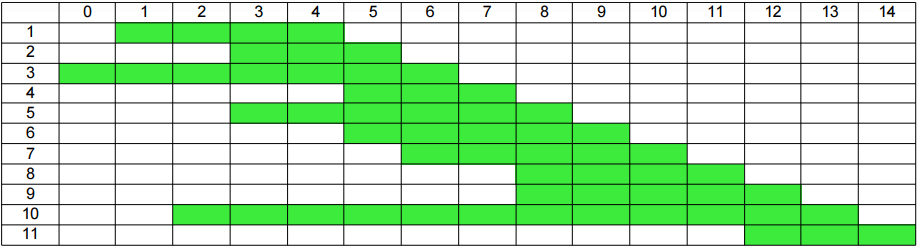
\includegraphics[width=.5\textwidth]{selecao}
\caption{Figura representando a seleção de 11 atividades em 14 unidades de tempo}
\label{fig:selecao}
\end{figure}

Assim, pode-se definir o problema matematicamente:

\begin{itemize}
\item Seja $S$ o conjunto de $n$ atividades que requerem o uso exclusivo de um recurso.
	\begin{itemize}
		\item $S = \{ a_{1}, a_{2}, ..., a_{n} \} $
	\end{itemize}
\item Cada atividade $a_{i}$ possui um tempo de início $s_{i}$ e um tempo de término $_{i}$, de forma que $0 \leq s_{i} < f_{i} < \infty $

\item A atividade $a_{i}$ será alocada no interfalo $ [ s_{i}, f_{i} ) $ se selecionada. 
\item Atividades $a_{i}$ e $a_{j}$ são mutuamente compatíveis se:
	\begin{itemize}
		\item $s_{i} \geq f_{j}$ ou $s_{j} \geq f_{i} $
	\end{itemize}
\end{itemize}

O problema da seleção das atividades possui diversas aplicações no dia-a-dia. As atividades podem ser encaradas como provas a serem executadas, e o recurso como uma única sala. Assim, dada uma lista de atividades o problema retorna o maior número de atividades que pode ser realizado em um espaço de tempo. Outra aplicação que usa esses conceitos é o agendamento de recursos computacionais realizado pelo Sistema Operacional.



Este trabalho tem como objetivo discutir e comparar a solução do problema da Seleção de atividades através de três algoritmos diferentes:
\begin{itemize}
\item Método Guloso
\item Programação Dinâmica
\item Backtracking
\end{itemize}

Os algoritmos serão comparados com base em seus resultados e tempo de execução, usando-se instâncias geradas aleatóriamente dos seguintes tamanhos:
\begin{itemize}
\item 10 atividades
\item 100 atividades
\item 1000 atividades
\item 10000 atividades
\end{itemize}

Ao final será demonstrado que a solução gulosa possui o melhor desempenho para este tipo de problema.

\section{Método Guloso} \label{sec:guloso}

Os métodos gulosos são um conjunto de métodos que fazem uso da heurística da melhor solução local em cada etapa de execução. Por conta desta característica, nem sempre garantem a solução ótima de um problema.

Para que a solução gulosa apresente uma solução ótima, deve possuir a característica de que cada escolha gulosa contenha uma solução ótima para o problema proposto, mostrando assim que o restante do problema também possui uma solução ótima.
O problema proposto possui uma subestrutura ótima, e portanto, existe um algoritmo guloso que o resolve de forma ótima

Neste trabalho, a implementação ótima foi realizada através do algoritmo abaixo:

 \begin{algorithm}[H]
   \SetAlgoLined
   \Entrada{$A$ Array contendo as atividades} 
   \Saida{Array contendo número máximo de atividades compatíveis entre si}
   \Inicio{
   		$ S \leftarrow \emptyset$ \\
   		$ A1 \leftarrow A$ ordenado em função de $s_{i}$\\
   		$ultima\_selecionada \leftarrow A1_{0}$ \\
    	\Para{cada $atividade \in A1$}{
    		\Se{ $atividade.inicio \geq ultima\_selecionada.fim $} {
    			$S \cup atividade$\\
    			$ ultima\_selecionada \leftarrow atividade $\\
    		}
     	}
   }
   \Retorna{$S$}
   \label{alg1}
   \caption{\textsc{Seleção de Atividades pelo método guloso}}
 \end{algorithm}

\subsection{Complexidade do algoritmo}
Analisando o algoritmo acima, pode-se perceber que a primeira etapa envolve a ordenação do vetor de atividades. Para tal, pode-se usar métodos de ordenação conhecidos, como o QuickSort, assim, a primeira etapa do algoritmo terá complexidade $O(n\log{}n)$ .

A segunda etapa consiste-se de uma busca sequencial por atividades mutuamente compatíveis, sendo portanto de complexidade $O(n)$ .

\begin{equation}
T(n) = O(n\log{}n) + O(n) = O(n\log{}n)
\end{equation}

\section{Programação Dinâmica}


\section{Backtracking}

\section{Resultados}

\section{Conclusão}

\bibliographystyle{sbc}
\bibliography{sbc-template}

\end{document}
